\documentclass[journal]{IEEEtran}

% *** CITATION PACKAGES ***
\usepackage{cite}

% *** GRAPHICS RELATED PACKAGES ***
%
\ifCLASSINFOpdf
\usepackage[pdftex]{graphicx}
  % declare the path(s) where your graphic files are
  % \graphicspath{{../pdf/}{../jpeg/}}
  % and their extensions so you won't have to specify these with
  % every instance of \includegraphics
  % \DeclareGraphicsExtensions{.pdf,.jpeg,.png}
\else
  % or other class option (dvipsone, dvipdf, if not using dvips). graphicx
  % will default to the driver specified in the system graphics.cfg if no
  % driver is specified.
  % \usepackage[dvips]{graphicx}
  % declare the path(s) where your graphic files are
  % \graphicspath{{../eps/}}
  % and their extensions so you won't have to specify these with
  % every instance of \includegraphics
  % \DeclareGraphicsExtensions{.eps}
\fi
% graphicx was written by David Carlisle and Sebastian Rahtz. It is
% required if you want graphics, photos, etc. graphicx.sty is already
% installed on most LaTeX systems. The latest version and documentation
% can be obtained at: 
% http://www.ctan.org/pkg/graphicx
% Another good source of documentation is "Using Imported Graphics in
% LaTeX2e" by Keith Reckdahl which can be found at:
% http://www.ctan.org/pkg/epslatex
%
% latex, and pdflatex in dvi mode, support graphics in encapsulated
% postscript (.eps) format. pdflatex in pdf mode supports graphics
% in .pdf, .jpeg, .png and .mps (metapost) formats. Users should ensure
% that all non-photo figures use a vector format (.eps, .pdf, .mps) and
% not a bitmapped formats (.jpeg, .png). The IEEE frowns on bitmapped formats
% which can result in "jaggedy"/blurry rendering of lines and letters as
% well as large increases in file sizes.
%
% You can find documentation about the pdfTeX application at:
% http://www.tug.org/applications/pdftex






% *** PDF, URL AND HYPERLINK PACKAGES ***
%
%\usepackage{url}
% url.sty was written by Donald Arseneau. It provides better support for
% handling and breaking URLs. url.sty is already installed on most LaTeX
% systems. The latest version and documentation can be obtained at:
% http://www.ctan.org/pkg/url
% Basically, \url{my_url_here}.


% correct bad hyphenation here
\hyphenation{op-tical net-works semi-conduc-tor}


\begin{document}
%
% paper title
% Titles are generally capitalized except for words such as a, an, and, as,
% at, but, by, for, in, nor, of, on, or, the, to and up, which are usually
% not capitalized unless they are the first or last word of the title.
% Linebreaks \\ can be used within to get better formatting as desired.
% Do not put math or special symbols in the title.
\title{Análisis de Sentimientos y Tendencias en Reseñas de Cafeterías en Google Maps}


\author{Álvaro Salgado López}

% note the % following the last \IEEEmembership and also \thanks - 
% these prevent an unwanted space from occurring between the last author name
% and the end of the author line. i.e., if you had this:
% 
% \author{....lastname \thanks{...} \thanks{...} }
%                     ^------------^------------^----Do not want these spaces!
%
% a space would be appended to the last name and could cause every name on that
% line to be shifted left slightly. This is one of those "LaTeX things". For
% instance, "\textbf{A} \textbf{B}" will typeset as "A B" not "AB". To get
% "AB" then you have to do: "\textbf{A}\textbf{B}"
% \thanks is no different in this regard, so shield the last } of each \thanks
% that ends a line with a % and do not let a space in before the next \thanks.
% Spaces after \IEEEmembership other than the last one are OK (and needed) as
% you are supposed to have spaces between the names. For what it is worth,
% this is a minor point as most people would not even notice if the said evil
% space somehow managed to creep in.








% If you want to put a publisher's ID mark on the page you can do it like
% this:
%\IEEEpubid{0000--0000/00\$00.00~\copyright~2015 IEEE}
% Remember, if you use this you must call \IEEEpubidadjcol in the second
% column for its text to clear the IEEEpubid mark.



% use for special paper notices
%\IEEEspecialpapernotice{(Invited Paper)}


\markboth{Procesamiento Y Clasificación de Datos, 23 Enero 2025}{}

% make the title area
\maketitle



%\IEEEpeerreviewmaketitle



\section{Introducción}
% The very first letter is a 2 line initial drop letter followed
% by the rest of the first word in caps.
% 
% form to use if the first word consists of a single letter:
% \IEEEPARstart{A}{demo} file is ....
% 
% form to use if you need the single drop letter followed by
% normal text (unknown if ever used by the IEEE):
% \IEEEPARstart{A}{}demo file is ....
% 
% Some journals put the first two words in caps:
% \IEEEPARstart{T}{his demo} file is ....
% 
% Here we have the typical use of a "T" for an initial drop letter
% and "HIS" in caps to complete the first word.
\IEEEPARstart
{E}{n} la era digital actual, las reseñas de usuarios se han convertido en una herramienta clave para comprender las percepciones del consumidor sobre productos y servicios. En particular, las reseñas de cafeterías proporcionan valiosa información sobre la experiencia de los clientes, que va más allá de las calificaciones numéricas. Sin embargo, procesar y analizar grandes cantidades de texto puede ser un desafío.

El objetivo de este análisis es explorar las reseñas de usuarios sobre cafeterías en Google Maps, con el fin de evaluar el sentimiento general que los consumidores tienen hacia diferentes establecimientos. A través del análisis de sentimiento, se busca clasificar las reseñas en categorías de sentimiento positivo, negativo y neutral. Este enfoque no solo ayudará a identificar cuáles son las cafeterías mejor valoradas por los usuarios, sino que también permitirá reconocer las características más mencionadas y asociadas a una mejor experiencia.

Para llevar a cabo este análisis, se utilizó una combinación de técnicas de procesamiento de lenguaje natural (PLN), como la vectorización de texto y el análisis de sentimiento. Estas herramientas permiten convertir las reseñas en datos cuantitativos que pueden ser fácilmente analizados para obtener conclusiones significativas. Además, se llevó a cabo un estudio de las palabras clave más relevantes dentro de las reseñas, con el fin de identificar patrones que influyen en las percepciones positivas y negativas de los clientes.
% You must have at least 2 lines in the paragraph with the drop letter
% (should never be an issue)

\section{Metodología}

El objetivo principal de este análisis es evaluar el sentimiento de los usuarios sobre diversas cafeterías de Monterrey utilizando reseñas publicadas en Google Maps. Para ello, se implementó un proceso que consta de varias fases, las cuales incluyen la recolección de datos, el preprocesamiento, la vectorización de texto y el análisis de sentimientos. A continuación, se describen en detalle los pasos seguidos:
\subsection{Recolección de datos}
Se recopiló un conjunto de reseñas de usuarios sobre cafeterías de Monterey de Google Maps. Las reseñas incluyen tanto comentarios positivos como negativos de los consumidores, los cuales contienen información valiosa sobre su experiencia en cada cafetería.
\subsection{Preprocesamiento de las reseñas}
Antes de realizar cualquier análisis, se llevó a cabo un proceso de limpieza y preprocesamiento de las reseñas. Este paso incluye la eliminación de caracteres no deseados, la conversión de las palabras a su forma base (lematización) y la eliminación de palabras vacías (stopwords) que no aportan significado relevante para el análisis de sentimiento.
\subsection{Vectorización de las reseñas}
Para convertir las reseñas en una forma que pueda ser procesada por los modelos de análisis, se utilizó un enfoque de vectorización. Se optó por utilizar el método de TF-IDF (Term Frequency-Inverse Document Frequency), que permite identificar las palabras más relevantes en relación con cada reseña. Este enfoque considera la frecuencia de las palabras en los documentos y ajusta su valor en función de su rareza en todo el conjunto de datos.
\subsection{Análisis de Sentimiento}
Con las reseñas preprocesadas y vectorizadas, se aplicó un modelo de análisis de sentimiento. En este caso, se utilizó un modelo de clasificación basado en un enfoque de aprendizaje automático para identificar si una reseña es positiva, negativa o neutral. El sentimiento de cada reseña se clasificó como “POSITIVE” o “NEGATIVE”, lo que permitió asignar un valor numérico (1 o -1) a cada reseña, facilitando el análisis posterior.
\subsection{Cálculo del Sentimiento Promedio por Cafetería}
Una vez clasificados los sentimientos, se calculó el promedio de los sentimientos para cada cafetería, permitiendo identificar las cafeterías con las reseñas más positivas y las más negativas. Este análisis se realizó a través de un agrupamiento por el nombre de la cafetería y calculando la media de los valores asignados a cada reseña.
\subsection{Visualización y Resultados}
Finalmente, se realizaron visualizaciones para mostrar las cafeterías con el mayor sentimiento positivo y negativo. Se generaron gráficos y tablas que presentan las cafeterías mejor valoradas y las menos favorecidas por los consumidores.

En resumen, el enfoque utilizado para este análisis combina técnicas de procesamiento de texto, aprendizaje automático y análisis estadístico para obtener una visión clara sobre las preferencias y la experiencia de los consumidores en diferentes cafeterías.

\section{Resultados}
En esta sección, se presentan los hallazgos obtenidos después de realizar el análisis de sentimiento sobre las reseñas de cafeterías en Google Maps. A partir del procesamiento y la clasificación de las reseñas, se pudo obtener información sobre las cafeterías con las mejores y peores valoraciones según el sentimiento de los usuarios.

El análisis de sentimiento permitió clasificar las reseñas en dos categorías: positivas y negativas. Las cafeterías fueron agrupadas y se calculó el promedio de los sentimientos de sus reseñas. El valor de sentimiento promedio para cada cafetería se presenta en una escala que va de -1 (negativo) a 1 (positivo). A continuación se presentan los resultados más relevantes:
\begin{itemize}
    \item Las cafeterías con un sentimiento promedio positivo son aquellas que obtuvieron una mayor proporción de reseñas favorables, reflejando una experiencia agradable para la mayoría de los usuarios. Estas cafeterías se destacan por ofrecer un servicio de calidad, buen ambiente y sabores que satisfacen las expectativas de los clientes.
    \item Las cafeterías con un sentimiento promedio negativo son aquellas con más reseñas desfavorables. Los usuarios indicaron su insatisfacción por aspectos como la calidad del café, el servicio al cliente o la falta de limpieza.
\end{itemize}

El análisis reveló un top 10 de cafeterías con el mejor sentimiento promedio. Este grupo de cafeterías se caracteriza por un alto índice de satisfacción, evidenciado por un sentimiento promedio igual a 1. Los usuarios comentaron positivamente sobre la calidad de los productos, la atención personalizada y la atmósfera relajada. Estas cafeterías están recomendadas por muchos de los consumidores, lo que les otorga una excelente reputación, en la Fig \ref{top10}
\begin{figure}
    \centering
    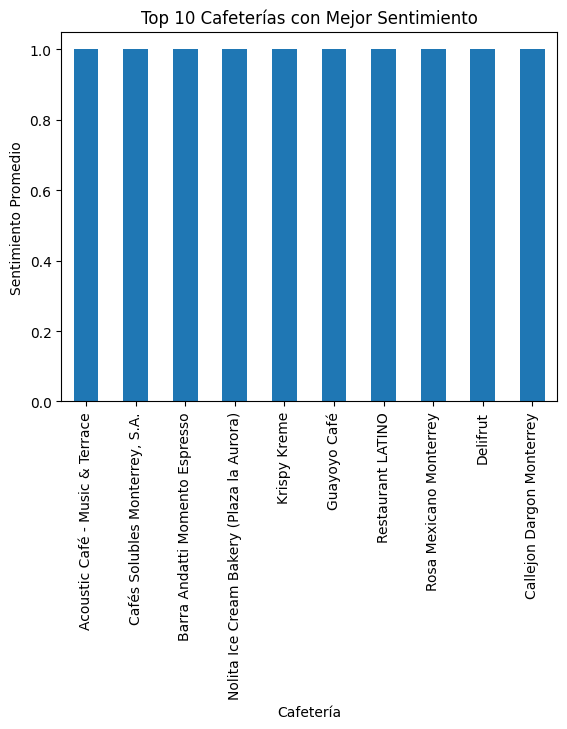
\includegraphics[width=0.5\linewidth]{Figs/top10.png}
    \caption{Cafeterías con promedio más alto}
    \label{top10}
\end{figure}

Por otro lado, también se identificaron cafeterías con el peor sentimiento promedio. Este grupo de establecimientos recibió numerosas críticas negativas, reflejadas en un sentimiento promedio cercano a -1 como puede observarse en la Fig \ref{peor10} Las reseñas mencionan principalmente deficiencias en el servicio, malos tratos por parte del personal o calidad deficiente en los productos. Estas cafeterías deberían considerar mejorar ciertos aspectos de su negocio para recuperar la satisfacción de los clientes.

\begin{figure}
    \centering
    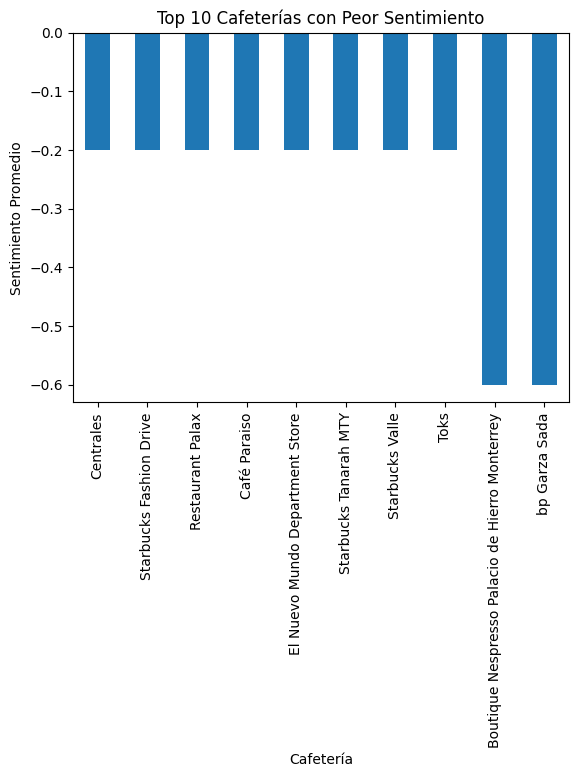
\includegraphics[width=0.5\linewidth]{Figs/peor10.png}
    \caption{Cafeterías con promedio mas bajo}
    \label{peor10}
\end{figure}
Para obtener las palabras más representativas en el conjunto de reseñas, se aplicó el cálculo de frecuencia inversa de documentos ponderada (TF-IDF). Este análisis revela las palabras que son más relevantes para todas las reseñas, considerando su frecuencia relativa y su dispersión a través de diferentes documentos.

Las palabras más importantes en el conjunto de reseñas de las cafeterías, junto con sus valores de TF-IDF, son las siguientes:
\begin{enumerate}
    \item good - 17.56
    \item coffee - 14.60
    \item great - 13.17
    \item place - 12.46
    \item service - 11.79
\end{enumerate}


Estas palabras reflejan los aspectos más relevantes de las reseñas, destacando atributos comunes como la calidad del “coffee” (café), el “service” (servicio), y la “food” (comida), los cuales son temas recurrentes en las opiniones de los usuarios.
\section{Conclusión}
En este análisis de sentimiento sobre las reseñas de cafeterías, hemos logrado identificar tanto las emociones predominantes como los aspectos clave que los clientes consideran más relevantes en sus evaluaciones. La metodología empleada, que incluyó el uso de técnicas de procesamiento de lenguaje natural (PLN) y la vectorización de texto mediante el cálculo de TF-IDF, permitió extraer información valiosa sobre los atributos de las cafeterías que influyen en la percepción de los clientes.

Al aplicar el análisis de sentimiento, se pudo observar que la mayoría de las reseñas tienen un tono positivo, lo que resalta la satisfacción de los clientes con respecto a la calidad del servicio, la comida, y el ambiente en las cafeterías. Este hallazgo es consistente con las palabras clave más destacadas, tales como “good”, “coffee”, “great”, y “service”, que son indicativas de una experiencia positiva.

Además, el análisis de las palabras más importantes en las reseñas nos proporcionó una visión clara de qué aspectos destacan los usuarios al describir sus experiencias, tales como el sabor del café, la calidad del servicio y el ambiente en general. Esta información es fundamental para las cafeterías, ya que les permite identificar áreas clave para mejorar y maximizar la satisfacción del cliente.

En resumen, este estudio no solo ofrece una visión detallada de las opiniones de los clientes, sino que también proporciona a los propietarios de cafeterías herramientas para evaluar y optimizar su servicio, mejorando así la experiencia del cliente y potencialmente incrementando su fidelidad.
% Can use something like this to put references on a page
% by themselves when using endfloat and the captionsoff option.
\ifCLASSOPTIONcaptionsoff
  \newpage
\fi



% trigger a \newpage just before the given reference
% number - used to balance the columns on the last page
% adjust value as needed - may need to be readjusted if
% the document is modified later
%\IEEEtriggeratref{8}
% The "triggered" command can be changed if desired:
%\IEEEtriggercmd{\enlargethispage{-5in}}

% references section

% can use a bibliography generated by BibTeX as a .bbl file
% BibTeX documentation can be easily obtained at:
% http://mirror.ctan.org/biblio/bibtex/contrib/doc/
% The IEEEtran BibTeX style support page is at:
% http://www.michaelshell.org/tex/ieeetran/bibtex/
%\bibliographystyle{IEEEtran}
% argument is your BibTeX string definitions and bibliography database(s)
%\bibliography{IEEEabrv,../bib/paper}
%
% <OR> manually copy in the resultant .bbl file
% set second argument of \begin to the number of references
% (used to reserve space for the reference number labels box)

%\bibliographystyle{IEEEtran} % Estilo de citas de IEEE
%\bibliography{referencias} % Nombre de tu archivo .bib


\end{document}


